\documentclass{article}

\usepackage{fancyhdr}
\usepackage{extramarks}
\usepackage{amsmath}
\usepackage{minted}
\usepackage{amsthm}
\usepackage{amsfonts}
\usepackage{tikz}
\usepackage[plain]{algorithm}
\usepackage{algpseudocode}

\usetikzlibrary{automata,positioning}
\usepackage{fullpage,enumitem,amsmath,amssymb,graphicx}

%
% Basic Document Settings
%

\topmargin=-0.75in
\textwidth=6.5in
\textheight=9.0in
\headsep=0.20in
\headheight = 12pt
\linespread{1.1}

\pagestyle{fancy}
\chead{\hmwkClass\ (\hmwkClassInstructor): \hmwkTitle}
\rhead{\firstxmark}
\lfoot{\lastxmark}
\cfoot{\thepage}

\renewcommand\headrulewidth{0.55pt}
\renewcommand\footrulewidth{0.55pt}

\setlength\parindent{0pt}


\setcounter{secnumdepth}{0}

%
% Homework Problem Environment
%
% This environment takes an optional argument. When given, it will adjust the
% problem counter. This is useful for when the problems given for your
% assignment aren't sequential. See the last 3 problems of this template for an
% example.

%
% Homework Details
%   - Title
%   - Due date
%   - Class
%   - Section/Time
%   - Instructor
%   - Author
%

\newcommand{\hmwkTitle}{Homework\ \#5}
\newcommand{\hmwkDueDate}{October 19, 2021}
\newcommand{\hmwkClassCode}{COT 5615}
\newcommand{\hmwkClass}{Math for Intelligent Systems}
\newcommand{\hmwkClassYear}{Fall 2021}
\newcommand{\hmwkClassInstructor}{Professor Kejun Huang}
\newcommand{\hmwkAuthorName}{\textit{Vyom Pathak}}
\newcommand{\hmwkUFID}{96703101}

%
%
%
% Various Helper Commands
%

% Useful for algorithms
\newcommand{\alg}[1]{\textsc{\bfseries \footnotesize #1}}

% For derivatives
\newcommand{\deriv}[1]{\frac{\mathrm{d}}{\mathrm{d}x} (#1)}

% For partial derivatives
\newcommand{\pderiv}[2]{\frac{\partial}{\partial #1} (#2)}

% Integral dx
\newcommand{\dx}{\mathrm{d}x}

% Alias for the Solution section header
\newcommand{\solution}{\textbf{\large Solution}}

% Probability commands: Expectation, Variance, Covariance, Bias
\newcommand{\E}{\mathrm{E}}
\newcommand{\Var}{\mathrm{Var}}
\newcommand{\Cov}{\mathrm{Cov}}
\newcommand{\Bias}{\mathrm{Bias}}

% norm bars
\newcommand{\norm}[1]{\left\lVert#1\right\rVert}

\begin{document}

\begin{center}
{\Large \hmwkClassCode\ \hmwkClass\ \hmwkClassYear\ \hmwkTitle}

\begin{tabular}{rl}
UFID: & \hmwkUFID \\
Name: & \hmwkAuthorName \\
Instructor: & \hmwkClassInstructor \\
Due Date: & \hmwkDueDate \\ 
% Collaborators: & [list all the people you worked with]
\end{tabular}
\end{center}

\section*{Problem 10.11}
\subsection*{Trace of matrix-matrix product}
\subsubsection*{Solution}
\begin{enumerate}[label=\alph*]
    \item Trace represents diagonal entries, thus trace of $A^TB$ can be shows as follows:
    \begin{align*}
        \sum\limits_{i=1}^m (A^TB)_{ii} = \sum\limits_{i=1}^m \sum\limits_{j=1}^n (A^T)_{ij}(B)_{ji} = \sum\limits_{i=1}^m \sum\limits_{j=1}^n A_{ij}B_{ij}
    \end{align*}
    The complexity of the algorithm is $2mn$ flops, as we only need $mn$ multiplications and $mn-1$ additions.
    \item The matrix $B^TA$ is the transpose of $A^TB$, so it has the same diagonal entries and same trace. Hence, $tr(B^TA)=tr(A^TB)$
    \item From (a), we can derive $A^TA$ as follows:
    \begin{align*}
        A^TA = \sum\limits_{i=1}^m \sum\limits_{j=1}^n A^2_{ij} = \norm{A}^2
    \end{align*}
    \item Here the following derivations shows the proof:
    \begin{align*}
        tr(BA^T) = \sum\limits_{i=1}^m (BA^T)_{ii} = \sum\limits_{i=1}^m \sum\limits_{j=1}^n (B)_{ij}(A^T)_{ji} = \sum\limits_{i=1}^m \sum\limits_{j=1}^n B_{ij}A_{ij}
    \end{align*}
\end{enumerate}
\section*{Problem 10.13}
\subsection*{Laplacian matrix of a graph}
\subsubsection*{Solution}
\begin{enumerate}[label=\alph*]
    \item The Dirichlet energy can be derived as follows:
    \begin{align*}
        v^TLv = v^TAA^Tv = (A^Tv)^T(A^Tv) = \norm{A^Tv}^2 = D(v)
    \end{align*}
    \item Each entry of $L_{ij}$ where $i=j$ i.e. $L_{ii}$ is the degree of node $i$ and when $i\neq j$ i.e. $L_{ij}$  is the negative of the number of edges between nodes $i$ and $j$. 
\end{enumerate}
\section*{Problem 10.31}
\subsection*{Diameter of a graph}
\subsubsection*{Solution}
\begin{enumerate}[label=\alph*]
    \item From the figure, it is clear that number of paths from j to i of length n is shown as $(A^k)_{ij}$. Thus, total number of paths of length no more than $k$ in-terms of $A$ can be shown as follows: $P = I + A + A^2 + A^3 + \ldots + A^k$
    \item Using equation from $(a)$, we can find the diameter by calculating $P$ for different values of $k$ until all the desired entries are positive and thus get the final result. 
\end{enumerate}
\section*{Problem 11.3}
\subsection*{Matrix cancellation}
\subsubsection*{Solution}
\begin{enumerate}[label=\alph*]
    \item $A = (1,0)^T,X = (0,1),\ and\ Y = (0,0)$
    \item Let $C$ be a left inverse of $A$, then by muliply $AX = AY$ on the left side by $C$ we get th following:\\ 
    $CAX = CAY \implies X = Y\ [\because CA = I]$ 
    \item As $A$ is non-invertible, its columns are linearly dependent i.e. $Ax = 0$ where $x$ is non-zero. Also, $Ay = 0$ where $y=0$. Thus, $Ax = Ay$ where $x\neq y$. Hence proved.
\end{enumerate}
\section*{Problem 11.11}
\subsection*{Interpolation of rational functions}
\subsubsection*{Solution}
The five interpolation equation can be written. as follows: 
    \begin{align*}
        c_1 + c_2 + c_3 & = 2(1 + d_1 + d_2)\\
        c_1 + 2c_2 + 4c_3 & = 5(1 + 2d_1 + 4d_2)\\
        c_1 + 3c_2 + 9c_3 & = 9(1 + 3d_1 + 9d_2)\\
        c_1 + 4c_2 + 16c_3 & = -1(1 + 4d_1 + 16d_2)\\
        c_1 + 5c_2 + 25c_3 & = -4(1 + 5d_1 + 25d_2)\\
    \end{align*}
These equations can be represented in matrix form as follows:
\begin{align*}
(1,1,1,1,1;1,2,3,4,5;1,4,9,16,25;-2,-10,-27,4,20;-2,-20,-81,16,100)(c_1,c_2,c_3,d_1,d_2) = (2,5,9,-1,-4)
\end{align*}

The solution of the above equation is:
\begin{align*}
c_1 = 0.62962,\ c_2 = 0.60493,\ c_3 =-0.19753,\ d_1 =-0.56790,\ d_2 =0.08641
\end{align*}
The figure~\ref{fig:inter} shows the given rational function with the solution points.
\begin{figure}
    \centering
    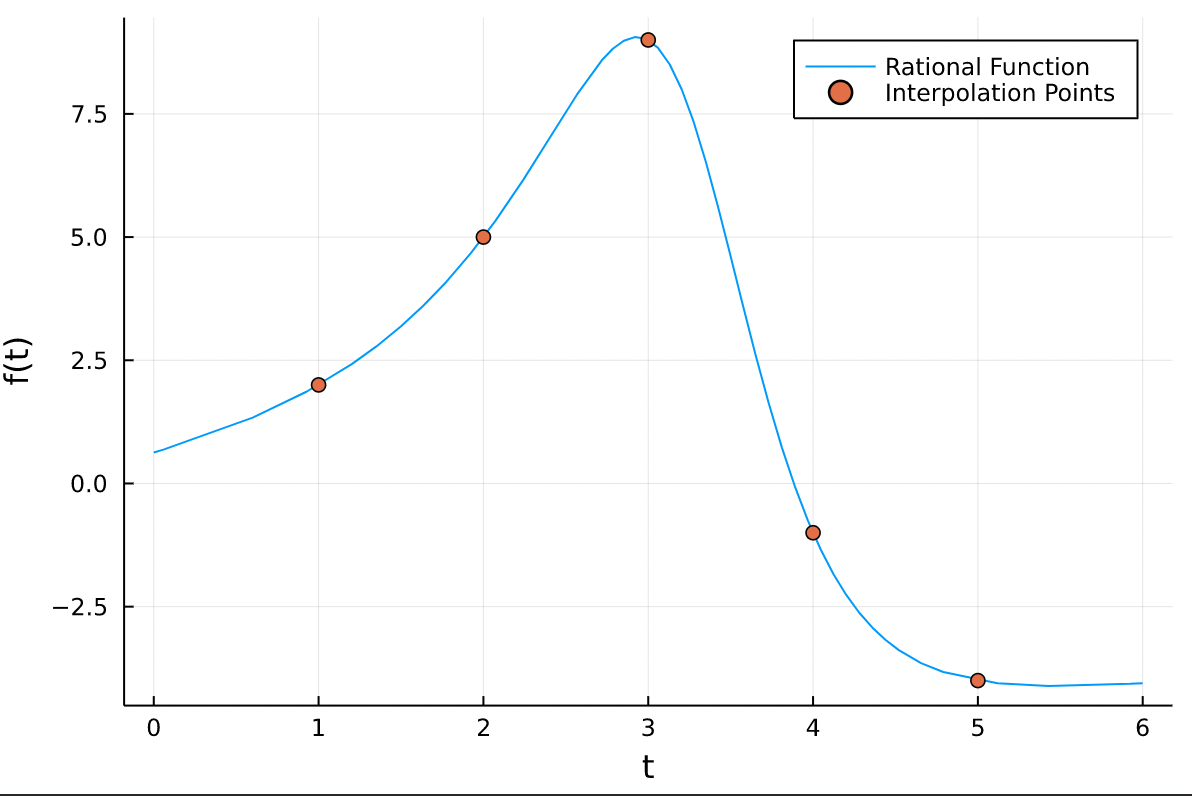
\includegraphics[width=0.75\textwidth]{Interpolation_Rational_Function.png}
    \caption{Interpolation of Rational Function}
    \label{fig:inter}
\end{figure}
\begin{minted}[
frame=lines,
framesep=2mm,
baselinestretch=1.2,
fontsize=\footnotesize,
linenos
]{julia}
    using Plots
    using LinearAlgebra
    Plots.PlotlyBackend()
    A = [1 1 1 1 1;1 2 3 4 5;1 4 9 16 25;-2 -10 -27 4 20;-2 -20 -81 16 100]';
    C = [2 5 9 -1 -4]';
    B = inv(A)C;
    display(B);
    f(t) = ((B[1])+(B[2]*t)+(B[3]*t*t))/(1+(B[4]*t)+(B[5]*t*t));
    plot(f, 0, 6,label = "Rational Function",xlabel="t",ylabel="f(t)")
    scatter!([1,2,3,4,5],[2,5,9,-1,-4],label="Interpolation Points")
    \end{minted}
\section*{Problem 11.21}
\subsection*{Quadrature weights.}
\subsubsection*{Solution}
\begin{align*}
    (1,t_1,t^2_1,t^3_1;1,t_2,t^2_2,t^3_2;1,t_3,t^2_3,t^3_3;1,t_4,t^2_4,t^3_4)\ (w_1,w_2,w_3,w_4) = (b_1,b_2,b_3,b_4)
\end{align*}
Here $t_i$ where $i=1\ldots 4$ are the values of the vector $t=(-0.6, -0.2, 0.2, 0.6)$, and 
\begin{align*}
    b_k = \int\limits_{-1}^{1} t^{k-1}dt = \begin{cases}
  2/k & k\ is\ odd\\    
  0 k & k\ is\ even
\end{cases}
\end{align*}
By solving it using left-inverse and matrix multiplication, we get the following values of w:
\begin{align*}
    w_1 = 0.9166\ ,\ w_2 = 0.0833\ ,\ w_3=0.0833\ ,\ w_4 = 0.9166
\end{align*}
Furthermore, for solving $f(t)=e^x$ we get the following values:
\begin{align*}
    \alpha = 2.3504\ ,\ \hat{\alpha}=2.3433
\end{align*}
Following is the code for the above calculation:
\begin{minted}[
frame=lines,
framesep=2mm,
baselinestretch=1.2,
fontsize=\footnotesize,
linenos
]{julia}
    A = [1 1 1 1; -0.6 -0.2 0.2 0.6; (-0.6)^2 (-0.2)^2 (0.2)^2 (0.6)^2; (-0.6)^3 (-0.2)^3 (0.2)^3 (0.6)^3];
    b = [2 0 (2/3) 0]';
    W = A\b;
    f(x) = exp(x);
    alpha_cap = f.([-0.6 -0.2 0.2 0.6])*W;
    alpha = exp(1)-exp(-1);
    display(W);
    display(alpha_cap);
    display(alpha);
    \end{minted}
\end{document}
